\begin{table}[h]
\centering
\caption{Resultados dos cenários simulados no sistema Mamdani}
\label{tab:mamdani-resultados}
\begin{tabular}{|c|c|c|c|c|}
\hline
Cenário & Entrada & Centroide & Média do Máximo & Bissetriz \\
\hline
1 & (28, 80, 15) & forte & forte & forte \\
2 & (22, 50, 5)  & moderada & moderada & moderada \\
3 & (18, 30, 2)  & fraca & fraca & fraca \\
4 & (32, 60, 10) & forte & forte & forte \\
5 & (25, 90, 8)  & forte & forte & forte \\
\hline
\end{tabular}
\end{table}

\begin{figure}[htbp]
\centering
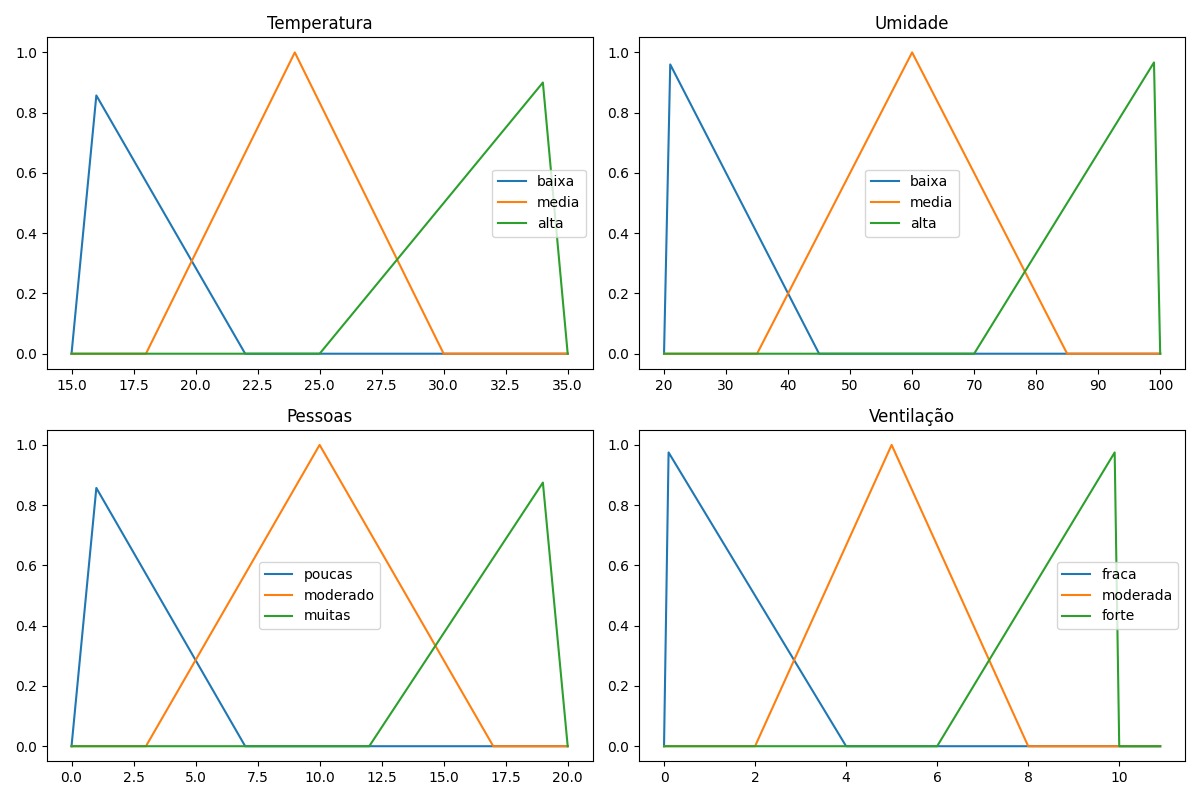
\includegraphics[width=0.9\linewidth]{../img/funcoes_pertinencia_mamdani2.png}
\caption{Funções de pertinência das variáveis do sistema Mamdani.}
\label{fig:pertinencia-mamdani}
\end{figure}

\begin{figure}[htbp]
\centering
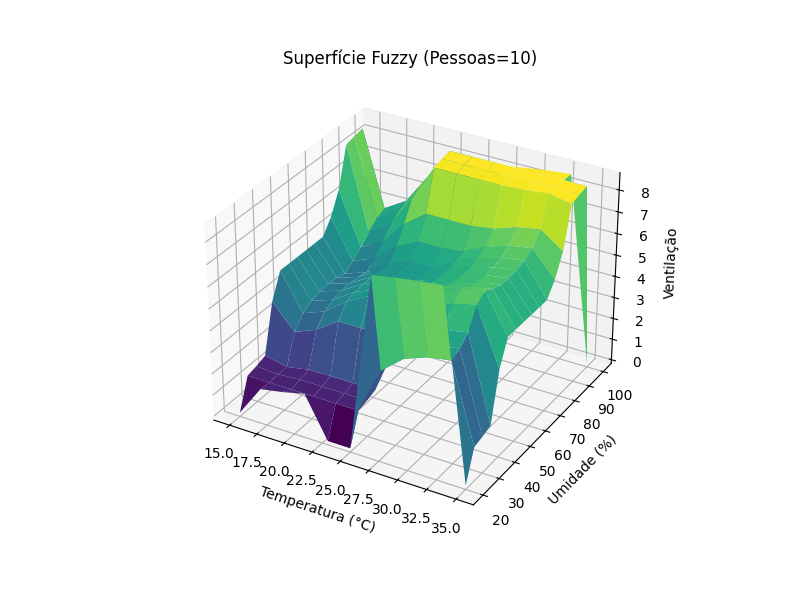
\includegraphics[width=0.9\linewidth]{../img/superficie_fuzzy_pessoas10_mamdani2.png}
\caption{Superfície fuzzy: ventilação em função de temperatura e umidade (pessoas=10).}
\label{fig:superficie-mamdani}
\end{figure}

\begin{figure}[htbp]
\centering
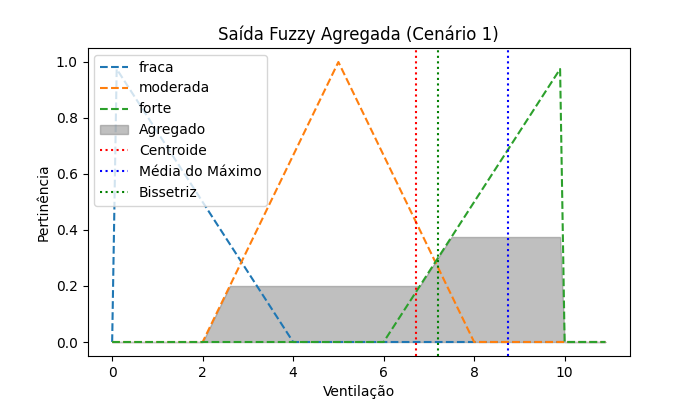
\includegraphics[width=0.9\linewidth]{../img/saida_fuzzy_cenario1_mamdani2.png}
\caption{Saída fuzzy agregada e defuzzificação para o cenário 1.}
\label{fig:saida-cenario1}
\end{figure}

\subsection{Sistema Takagi-Sugeno}

A aproximação da função $f(x)$ foi realizada utilizando sistemas de ordem zero e primeira ordem, além de diferentes funções de pertinência e operadores. Os principais resultados são:

\begin{itemize}
    \item \textbf{Ordem zero (gaussiana + produto):} RMSE $\approx$ 0.46
    \item \textbf{Ordem zero (triangular + produto):} RMSE $\approx$ 0.35
    \item \textbf{Ordem zero (trapezoidal + produto):} RMSE $\approx$ 0.35
    \item \textbf{Ordem zero otimizada (gradiente descendente):} RMSE $\approx$ 0.41
    \item \textbf{Primeira ordem (gaussiana):} RMSE $\approx$ 0.41
\end{itemize}

\begin{figure}[htbp]
\centering
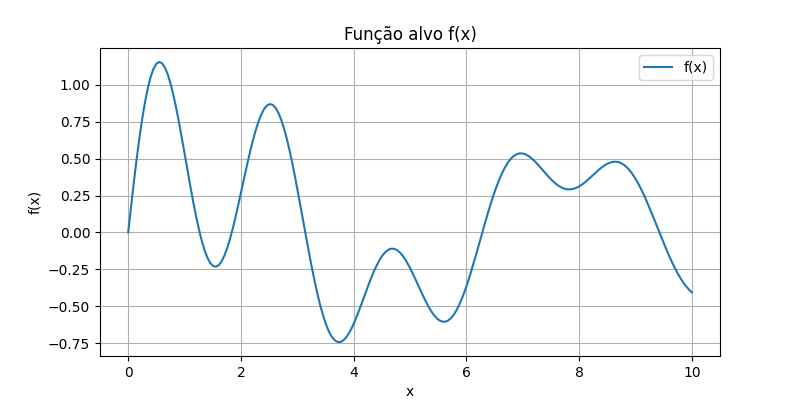
\includegraphics[width=0.9\linewidth]{../img/fx_takagi_sugeno2.png}
\caption{Função alvo $f(x)$ a ser aproximada pelo sistema Takagi-Sugeno.}
\label{fig:fx-takagi}
\end{figure}

\begin{figure}[htbp]
\centering
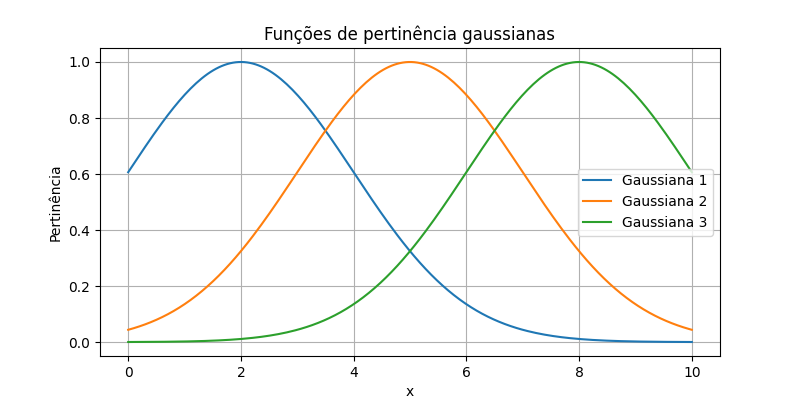
\includegraphics[width=0.9\linewidth]{../img/mfs_gauss_takagi_sugeno2.png}
\caption{Funções de pertinência gaussianas para o sistema Takagi-Sugeno.}
\label{fig:mf-gauss}
\end{figure}

\begin{figure}[htbp]
\centering
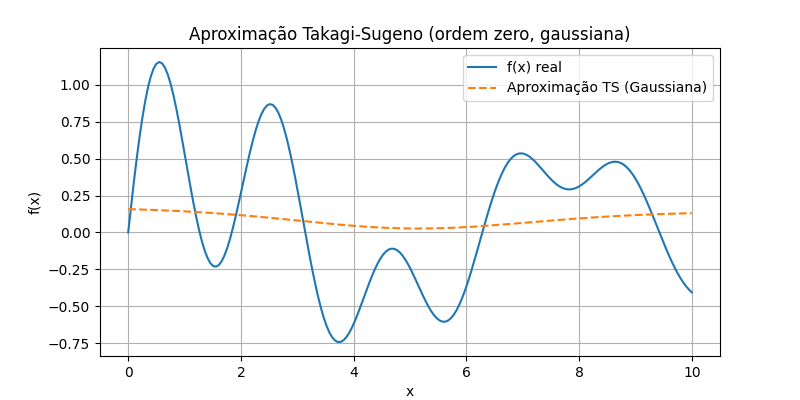
\includegraphics[width=0.9\linewidth]{../img/fx_aprox_gauss_takagi_sugeno2.png}
\caption{Aproximação Takagi-Sugeno (ordem zero, gaussiana).}
\label{fig:ts-gauss}
\end{figure}

\begin{figure}[htbp]
\centering
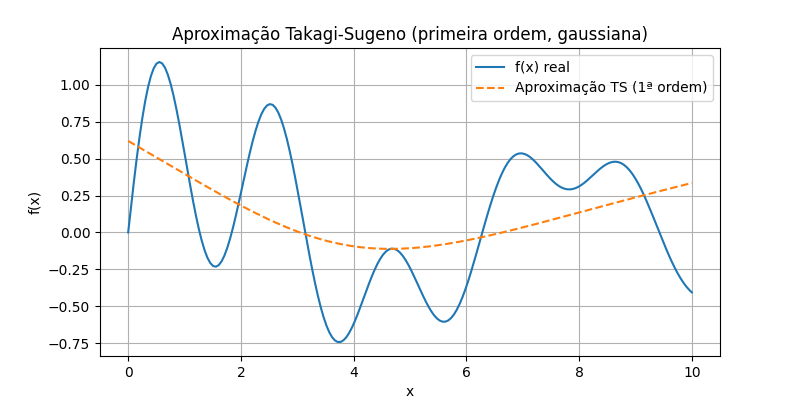
\includegraphics[width=0.9\linewidth]{../img/fx_aprox_1ordem_takagi_sugeno2.png}
\caption{Aproximação Takagi-Sugeno (primeira ordem, gaussiana).}
\label{fig:ts-1ordem}
\end{figure}

\begin{figure}[htbp]
\centering
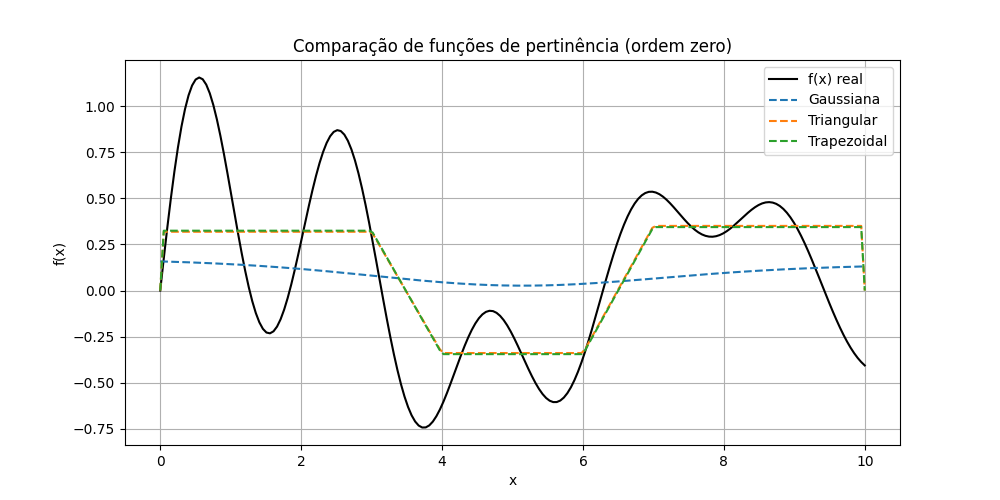
\includegraphics[width=0.9\linewidth]{../img/fx_aprox_comparacao_takagi_sugeno2.png}
\caption{Comparação de funções de pertinência (ordem zero).}
\label{fig:ts-comparacao}
\end{figure}

\begin{figure}[htbp]
\centering
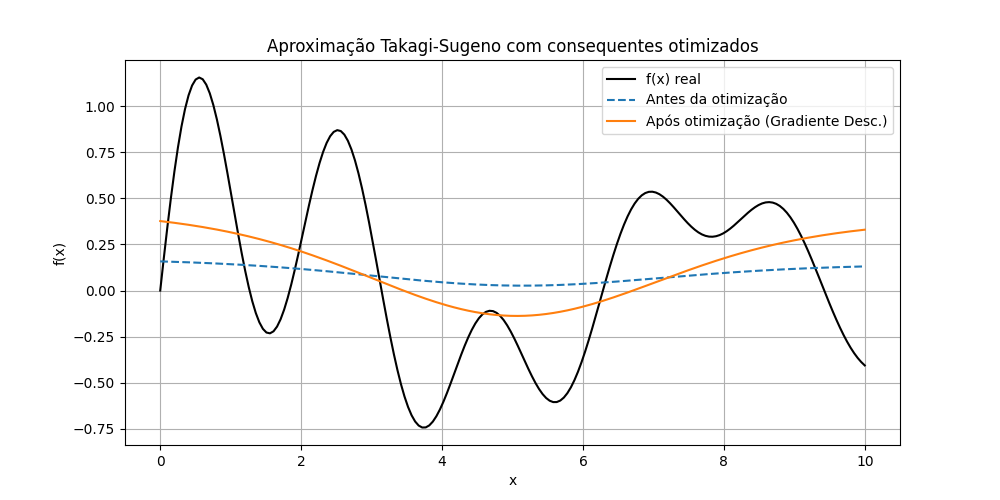
\includegraphics[width=0.9\linewidth]{../img/fx_aprox_otimizado_takagi_sugeno2.png}
\caption{Aproximação Takagi-Sugeno com consequentes otimizados (gradiente descendente).}
\label{fig:ts-otimizado}
\end{figure}

\begin{figure}[htbp]
\centering
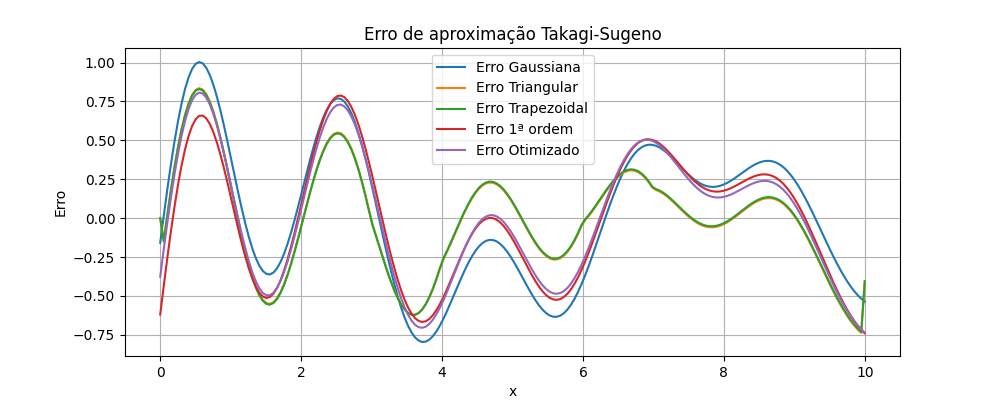
\includegraphics[width=0.9\linewidth]{../img/erro_takagi_sugeno2.png}
\caption{Erro de aproximação do sistema Takagi-Sugeno para cada configuração.}
\label{fig:ts-erro}
\end{figure}

\subsection{Visualização dos Resultados}

\begin{itemize}
    \item Gráficos das funções de pertinência para todas as variáveis (Fig.~\ref{fig:pertinencia-mamdani}, Fig.~\ref{fig:mf-gauss}).
    \item Superfície fuzzy (Fig.~\ref{fig:superficie-mamdani}).
    \item Saída fuzzy agregada e defuzzificação (Fig.~\ref{fig:saida-cenario1}).
    \item Aproximação da função $f(x)$ e erro para cada configuração testada (Fig.~\ref{fig:fx-takagi}, Fig.~\ref{fig:ts-gauss}, Fig.~\ref{fig:ts-1ordem}, Fig.~\ref{fig:ts-comparacao}, Fig.~\ref{fig:ts-otimizado}, Fig.~\ref{fig:ts-erro}).
\end{itemize}
